\chapter{More about Slurm}

In addition to the three main components (Slurmctld, Slurmdbd, Slurmd) mentioned in Section \ref{Sec:jobScheduler}, Figure \ref{fig_slurm_overview} shows the general slum architecture.

Slurm also adopts the plugin-based architecture. These plugins, from network topologies to authentication mechanisms, offer a customizable framework adaptable to different computing environments. Moreover, Slurm's robust plugin design allows for seamless integration of custom functionalities, empowering users to tailor the system to their specific needs.

This Chapter introduces Slurm's login-node commands and Slurm's key features. We also compare Slurm with Kubernetes.

\begin{figure}[tb]
    \centering
    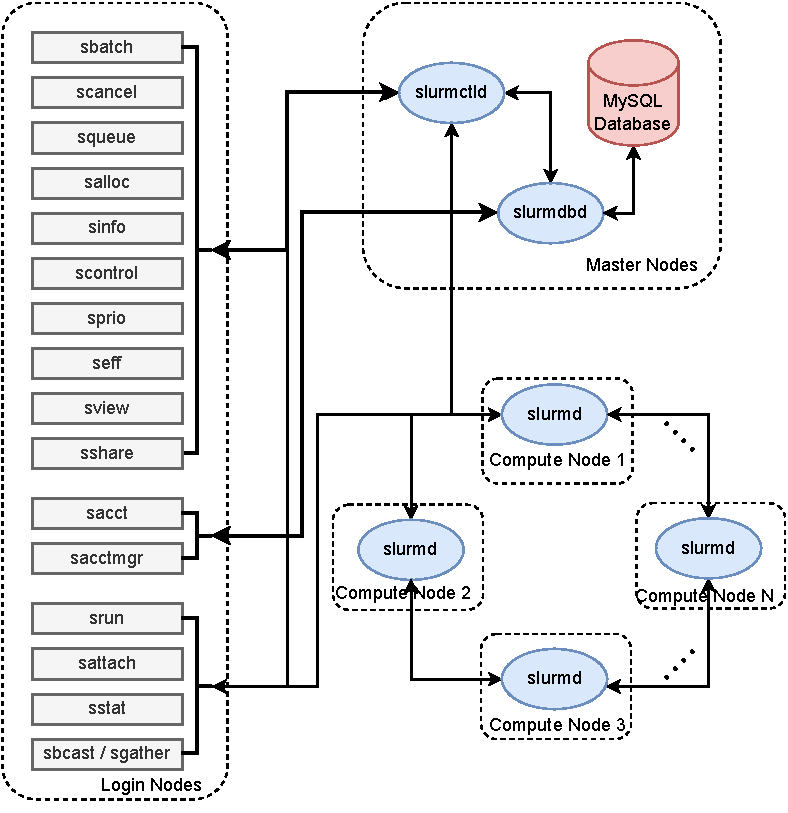
\includegraphics[width=0.8\textwidth]{figures/slurm-overview.pdf}
    \caption{Slurm architecture overview}
    \label{fig_slurm_overview}
\end{figure}



\section{Login-node commands}

Here are the available Slurm commands for users to interact in the login node:

\begin{itemize}
    \item \textbf{sbatch}: For submitting batch scripts, which can be written in bash, Perl, or Python, enabling users to automate the execution of tasks in a batch mode.
    \item \textbf{scancel}: Enabling the cancellation of pending or running jobs or job steps, providing users with control over job management and resource allocation.
    \item \textbf{squeue}: For querying pending and running jobs, providing users with visibility into the status of their submitted tasks and overall system workload.
    \item \textbf{salloc}: Users can interactively access computing resources for their tasks to request interactive job allocations.
    \item \textbf{sinfo}: Retrieving comprehensive information about partitions, reservations, and the state of nodes within the system, helping users understand the availability and status of computing resources.
    \item \textbf{scontrol}: Enabling users to manage jobs, query system configurations, and retrieve resource utilization and allocation information.
    \item \textbf{sprio}: Enabling users to query job priorities, assisting in resource allocation decisions and prioritization of tasks based on predefined criteria.
    \item \textbf{seff}: Providing a concise overview of resource utilization for active and completed batch jobs, detailing the requested and actual usage of resources.
    \item \textbf{sview}: GUI that offers state information for jobs, partitions, and nodes, enhancing user experience in monitoring and managing computing resources.
    \item \textbf{sshare}: Providing users with fair-share information, offering insights into resource allocation fairness among different users based on usage history and system policies.
    \item \textbf{sacct}: Retrieving accounting information about jobs and job steps stored in Slurm's database, assisting in resource usage analysis, billing, and reporting.
    \item \textbf{sacctmgr}: Enabling users to query accounting-related information and other accounting data stored in Slurm's database, facilitating user accounting management and administration tasks.
    \item \textbf{srun}: Initiating job steps, primarily within a job or starting interactive jobs, allowing for executing multiple steps sequentially or in parallel on allocated nodes within the job's resource allocation.
    \item \textbf{sattach}: Attaching standard input, output, and error streams, along with signal capabilities, to a currently running job or job step, facilitating real-time monitoring and interaction.
    \item \textbf{sstat}: Querying status information about running jobs, providing real-time updates on job progress, resource utilization, and other relevant metrics.
    \item \textbf{sbcast}: Facilitating the transfer of files to all nodes allocated for a specific job, so that we can ensure necessary data or resources to be available across the computing environment.
    \item \textbf{sgather}: Allowing the retrieval of files from all allocated nodes to the currently active job, serving as a mechanism for aggregating results or data produced during job execution.
\end{itemize}

\section{Key features}
Key features for Slurm include:
\begin{itemize}
    \item \textbf{High-availability} for the primary daemons, namely Slurmctld and Slurmdbd, ensuring uninterrupted operation.
    \item Compute nodes are grouped into \textbf{partitions} by Slurm, allowing for configuring various limits and policies for each partition, such as permitted users, maximum nodes, and maximum wall-time limit per job.
    \item \textbf{Quality-of-Services (QoS)} enforce additional limits based on the status of the user's group.
    \item Utilization of the \textbf{backfilling scheduling algorithm} to optimize job scheduling and enhance resource utilization.
    \item Job scheduling based on \textbf{priorities} allows efficient allocation according to user-defined criteria.
    \item \textbf{Accounting} mechanism utilizing Slurmdbd and the MySQL/MariaDB database to track resource usage and job statistics for Trackable RESources (TRES). Default TRES include nodes, CPUs, memory, and billing.
    \item \textbf{No preemption} policies support, meaning that administrators can configure Slurm so that running jobs are not subject to interruption.
    \item \textbf{Prologue and Epilogue} scripts to execute tasks before and after job execution.
    \item \textbf{Generic RESources (GRES)} such as GPUs and NVMe allow flexibility but lack built-in accounting support.
\end{itemize}

\section{With Kubernetes}

With the rise of cloud computing, container orchestration systems such as Kubernetes become increasingly popular. However, these tools are unsuitable for deployment in the HPC world, as HPC job schedulers like Slurm revolve around job completion. At the same time, Kubernetes is tailored for hosting and sustaining services over time \cite{9235080}. To be more precise, the primary distinction between an HPC workload and the typical application suited for Kubernetes lies in their operational characteristics. HPC workloads focus on efficiently executing a complex task within the shortest time frame, even if the duration is considerable. Conversely, Kubernetes excels in managing continuously running applications, particularly those designed as services.

However, there is a growing interest in integrating batch job systems with Kubernetes to provide the best of both worlds. Such integration aims to leverage Kubernetes's capabilities in managing scalable, long-running services while benefiting from the efficient scheduling and resource management of HPC systems like Slurm. Several models have been proposed for converging these environments, including \textit{Adjacent} and \textit{Under} models. In the \textit{Adjacent} model, both control planes are overlapped, with Slurm managing both traditional HPC and Kubernetes workloads, utilizing Kubernetes' capabilities like sidecars and operators. The \textit{Under} model involves running Slurm clusters within a Kubernetes environment, allowing for traditional user experiences and higher throughput for MPI workloads. At the same time, Kubernetes manages scaling and dynamic resource allocation. One such example project is SUNK (Slurm on Kubernetes) \cite{SlurmK8sIntegration}, which is working towards seamless integration to support large-scale AI training, as well as inference and other complex workflows on hybrid environments that combine cloud-native and HPC.